\documentclass{article}
\usepackage[margin=0.75in]{geometry}
\usepackage{fancyhdr}
\pagestyle{fancy}
\lhead{}
\chead{}
\rhead{Warren D. (Hoss) Craft HW 04 CS 561}
\lfoot{}
\cfoot{\thepage}
\rfoot{}
\usepackage{amsmath, amsthm, amssymb}
\usepackage{mathtools}
\usepackage{graphicx}
\usepackage{caption}
\usepackage{hyperref}
\usepackage{changepage}
\usepackage{lipsum}
\usepackage{scrextend} % for block indents (for example)
\usepackage{color, colortbl} % For Coloring Table Elements
\usepackage{listings}
\usepackage{makecell}  % allows more complex table formatting
\usepackage{multirow}
\usepackage{proof}     % for inference trees
\usepackage{subcaption}
\usepackage{enumitem}  % allows customization of enumerate

\usepackage{wrapfig}   % allows wrapping text around figures
\usepackage{sidecap}   % allows side captions on figures
\sidecaptionvpos{figure}{t}
\usepackage{physics}   % provides abs{} and norm{}

% for the makecell package:
\renewcommand\theadalign{bc}
\renewcommand\theadfont{\bfseries}
\renewcommand\theadgape{\Gape[4pt]}
\renewcommand\cellgape{\Gape[4pt]}

\addtolength{\hoffset}{-1cm}
\addtolength{\textwidth}{1cm}
\graphicspath{ {IMAGES/} }

\definecolor{Gray}{gray}{0.9}
\newcolumntype{g}{>{\columncolor{Gray}}c}

% for bibliography and citations
% see https://www.overleaf.com/learn/latex/Bibliography_management_in_LaTeX
% for usage details
\usepackage[
backend=biber,
style=numeric,
citestyle=numeric,
sorting=ynt
]{biblatex}
\addbibresource{bibliography.bib}

% for script lettering, e.g.
% for Fourier transform
\usepackage[mathscr]{euscript}

\usepackage{changepage} % for the adjustwidth environment
% For shading paragraph boxes
\usepackage[framemethod=tikz]{mdframed}

% tweak the style of nested enumerated lists
% to use italicized alpha characters
\renewcommand{\labelenumii}{(\textit{\alph{enumii}})}

\title{CS 561: Algorithms \& Data Structures\\
Homework 04}
\author{Warren D. (Hoss) Craft}
\date{Fall 2020 (due Mon 10/26/20)}

\begin{document}
\maketitle
%\tableofcontents

\flushleft

\textit{Preamble:} Space here for some notes, before the enumerated problems below. See end of document for example Figures and Tables. While we're at it, here's an example citation from the bibliography: Cormen \cite{Cormen_Algorithms:2009}

\begin{enumerate}[label=\textbf{(\arabic*)}]

%%%%%%%%%%%%%%%%%
%   Problem 1   %
%%%%%%%%%%%%%%%%%

\item Consider the following alternative greedy algorithms for the activity selection problem discussed in class. For each algorithm, either prove or disprove that it constructs an optimal schedule.

  \begin{enumerate} % Begin Sub-problems
  
    \item Choose an activity with shortest duration, discard all conflicting activities and recurse.
    
    \item Choose an activity that starts first, discard all conflicting activities and recurse.
    
  \end{enumerate} % End Sub-problems

\vspace{0.1in}

%%%%%%%%%%%%%%%%%%%%%%%%%%%
%   Problem 1 Solutions   %
%%%%%%%%%%%%%%%%%%%%%%%%%%%

\textbf{\textit{Solutions.}}

  \begin{enumerate} % Begin Sub-problems
    \item \textit{Shortest Duration.} Consider Figure (\ref{fig:Example_Figure_01}), showing a collection of ``disjoint in time'' activities $a_1, a_2, a_3, a_4, a_5$, all approximately equal in duration and a special activity $a^{\prime}$ of noticeably shorter duration \ldots .
    
    \vspace{0.1in}
    
    \begin{figure}[hbtp]
    \captionsetup{font=small, width = 10cm}
    \centering
       \centering
       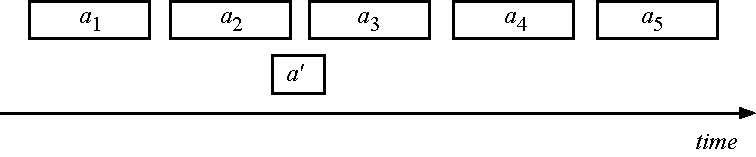
\includegraphics[width = 0.5\textwidth]{FIGURES/Example_Figure_01.pdf}
    \caption{See Problem 1(\textit{a}). Add more text here for figure caption.}
    \label{fig:Example_Figure_01}
    \end{figure}
    
    \item \textit{Starts First.} Consider Figure (\ref{fig:Example_Figure_02}), showing a collection of activities $a_1, a_2, a_3, a_4, a_5, a^{\prime}$. The original ``Ends First'' greedy algorithm would produce the 3-element activity set $\{a_1, a_3, a_4\}$, but the ``Starts First'' greedy algorithm would produce the single-element activity set $\{a^{\prime}\}$. Clearly then, the ``Starts First'' greedy algorithm will not generally produce an optimal schedule.
    
    \begin{figure}[hbtp]
    \captionsetup{font=small, width = 10cm}
    \centering
       \centering
       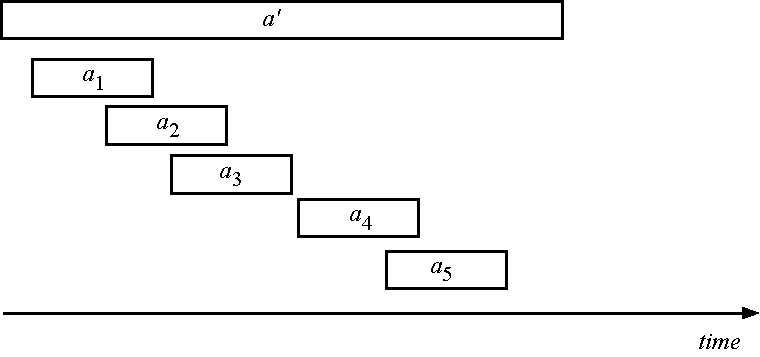
\includegraphics[width = 0.5\textwidth]{FIGURES/Example_Figure_02.pdf}
    \caption{See Problem 1(\textit{a}). A collection of activities where the ``Ends First'' greedy algorithm would produce the 3-element activity set $\{a_1, a_3, a_4\}$, but the ``Starts First'' greedy algorithm would produce the 1-element activity set $\{a^{\prime}\}$.}
    \label{fig:Example_Figure_02}
    \end{figure}
    
    \vspace{0.1in}
    
  \end{enumerate} % End Sub-problems

\vspace{0.1 in}

\clearpage

%%%%%%%%%%%%%%%%%
%   Problem 2   %
%%%%%%%%%%%%%%%%%

\item Second problem starts here.

  \begin{enumerate} % Begin Sub-problems
  
    \item Start sub-problem here.
    
    \vspace{0.1in}
    
    \item Start sub-problem here.
    
  \end{enumerate} % End Sub-problems

\vspace{0.1in}

%%%%%%%%%%%%%%%%%%%%%%%%%%%
%   Problem 2 Solutions   %
%%%%%%%%%%%%%%%%%%%%%%%%%%%

\textbf{\textit{Solutions.}}
  \begin{enumerate} % Begin Sub-prob solns
  
    \item Solution to 2(\textit{a}): \ldots.
    
    \vspace{0.1in}
    
    \item Solution  to 2(\textit{b}): \ldots.

  \end{enumerate} % End Sub-prob solns

\vspace{0.1in}

\clearpage

\end{enumerate}

EXAMPLES for use elsewhere \ldots

%%%%%%%%%%%%%%%%%%%%%%%%%%%%%%%%%
%   Example Aligned Equations   %
%   with Cases                  %
%%%%%%%%%%%%%%%%%%%%%%%%%%%%%%%%%

\begin{align}
        m(j)
        &=
        \max{}
        \begin{cases}
        m(x_j) + v_j\\
        m(j-1)
        \end{cases}
\end{align}

%%%%%%%%%%%%%%%%%%%%%%
%   Example Figure   %
%%%%%%%%%%%%%%%%%%%%%%

\begin{figure}[hbtp]
    \captionsetup{font=small, width = 10cm}
    \centering
       \centering
       \includegraphics[width = 0.5\textwidth]{FIGURES/HW04_1a.pdf}
    \caption{An example figure without subfigures.}
    \label{fig:Example_Figure_Without_Subfigures}
\end{figure}

%%%%%%%%%%%%%%%%%%%%%%%%%%%%%%%
%   Example Figure            %
%   Containing 2 Subfigures   %
%%%%%%%%%%%%%%%%%%%%%%%%%%%%%%%

\begin{figure}[htb]
\captionsetup{width = 15cm}
\centering
  \begin{subfigure}[b]{0.4\textwidth}
  \centering
  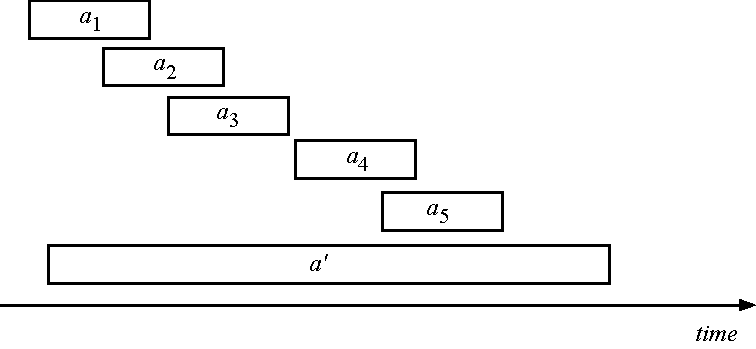
\includegraphics[width = 0.9\textwidth]{FIGURES/Example_Figure_03.pdf}
  \caption{Caption for subfigure (a).}
  \end{subfigure}
  \begin{subfigure}[b]{0.4\textwidth}
  \centering
  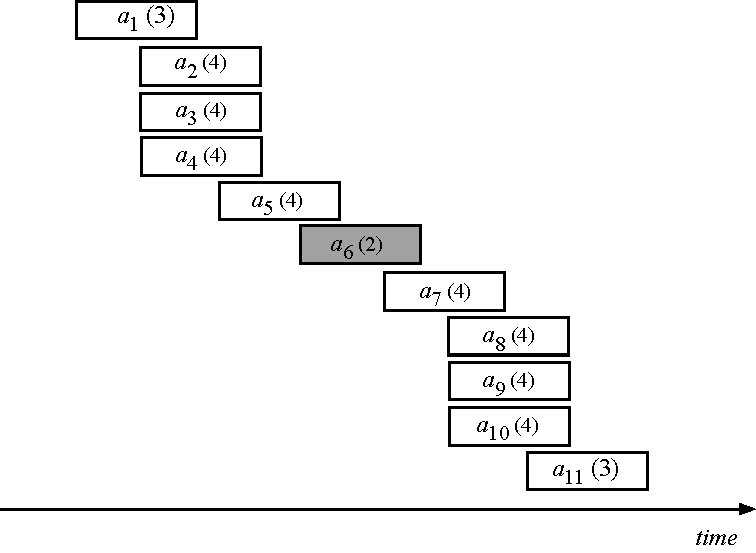
\includegraphics[width = 0.9\textwidth]{FIGURES/Example_Figure_04.pdf}
  \caption{Caption for subfigure (b).}
\end{subfigure}
\caption{Example Figure containining two sub-figures.}
\label{fig:Example_Figure_With_Two_Subfigures}
\end{figure}

%%%%%%%%%%%%%%%%%%%%%%%%%%%%%%%
%   Example Figure            %
%   Containing 2 Subfigures   %
%   Which Contain Tables      %
%%%%%%%%%%%%%%%%%%%%%%%%%%%%%%%

\begin{figure}[htb]
\captionsetup{width = 15cm}
\centering
  \begin{subfigure}{0.4\textwidth}
  \centering
  \begin{tabular}{c|c|c|c|c|}
         $r_i / c_j$ & \textbf{1} & \textbf{2} & \textbf{1} & \textbf{2}\\[5pt]
         \hline
         &&&&\\[-5pt]
         \textbf{1} & 0 & 0 & 1 & 0 \\[5pt]
         \hline
         &&&&\\[-5pt]
         \textbf{1}& 1 & 0 & 0 & 0 \\[5pt]
         \hline
         &&&&\\[-5pt]
         \textbf{2}& 0 & 1 & 0 & 1 \\[5pt]
         \hline
         &&&&\\[-5pt]
         \textbf{2} & 0 & 1 & 0 & 1 \\[5pt]
         \hline
    \end{tabular}
  \caption{}
  \end{subfigure}
  \begin{subfigure}{0.32\textwidth}
  \centering
  \begin{tabular}{c|c|c|c|c|}
         $r_i / c_j$ & \textbf{1} & \textbf{2} & \textbf{1} & \textbf{2}\\[5pt]
         \hline
         &&&&\\[-5pt]
         \textbf{1}& 0 & 1 & 0 & 0 \\[5pt]
         \hline
         &&&&\\[-5pt]
         \textbf{1}& 0 & 0 & 0 & 1 \\[5pt]
         \hline
         &&&&\\[-5pt]
         \textbf{2}& 1 & 1 & 0 & 0 \\[5pt]
         \hline
         &&&&\\[-5pt]
         \textbf{2}& 0 & 0 & 1 & 1 \\[5pt]
         \hline
    \end{tabular}
  \caption{}
\end{subfigure}
\caption{Example Figure containining two sub-figures, each containing a Table.}
\label{fig:Example_Figure_With_Two_Subfigure_Tables}
\end{figure}

% \clearpage
% ========== %
% END MATTER %
% ========== %
% \newpage

% For bibliography styles, see
% https://www.overleaf.com/learn/
% latex/Biblatex_bibliography_styles
% which is used in the preamble with the
% biblatex \usepackage command

\printbibliography

\end{document}